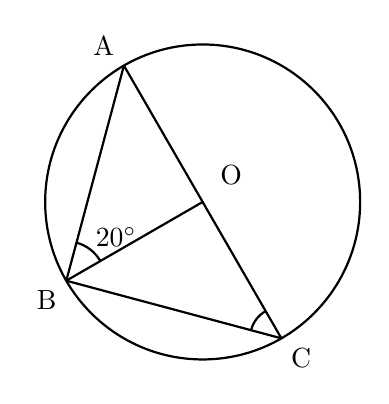
\begin{tikzpicture}[scale=1]

    % Define the center of the circle
    \coordinate (O) at (0,0);
    
    % Draw the main circle with a radius of 2cm
    \draw[thick] (O) circle (2cm);
    
    % Define coordinates for points A, B, and C on the circle
    % Using precise coordinates to ensure AC passes perfectly through O
    \coordinate (A) at (-1, 1.732);    % Angle 120 degrees
    \coordinate (B) at (-1.732, -1);   % Angle 210 degrees
    \coordinate (C) at (1, -1.732);    % Angle 300 degrees (exactly opposite to A)

    % Draw the line segment AC (diameter passing through the center O)
    \draw[thick] (A) -- (C);

    % Draw the line segment AB (chord)
    \draw[thick] (A) -- (B);

    % Draw the line segment BC (chord)
    \draw[thick] (B) -- (C);

    % Draw the line segment BO (radius connected precisely from B to O)
    \draw[thick] (B) -- (O);

    % Add an arc to indicate angle OBA
    % By using relative polar coordinates ++(angle:radius), the arc perfectly touches the lines
    % The angle of line BO is 30 degrees, and the angle of line BA is 75 degrees
    \draw[thick] (B) ++(30:0.5) arc (30:75:0.5);
    
    % Add the 20 degree label
    \node at (-1.1, -0.45) {$20^{\circ}$};

    % Add an arc to indicate angle BCA
    % The angle of line CA is 120 degrees, and the angle of line CB is 165 degrees
    \draw[thick] (C) ++(120:0.4) arc (120:165:0.4);

    % Add text labels exactly where they appear in the image
    \node[above right] at (0.1, 0.1) {O};
    \node[above left] at (A) {A};
    \node[below left] at (B) {B};
    \node[below right] at (C) {C};

\end{tikzpicture}